% status: 0
% chapter: Data

\title{Amazon Redshift}

\author{Karan Kotabagi}
\affiliation{%
  \institution{Indiana University}
 \streetaddress{School of Informatics, Computing, and Engineering}
  \city{Bloomington}
  \state{IN}
  \postcode{47404}
  \country{USA}}
\email{kkotabag@iu.edu}

\begin{abstract}
	Amazon Redshift is a quick, completely administered large-scale 
	information warehouse arrangement that enables the easy and 
	cost-effective solution to efficiently analyze expansive volumes 
	of information utilizing the existing tools of the business 
	intelligence. Amazon Redshift has been launched into the market in 
	February 2013. Since then, the service has grown to an innumerable 
	extent and has been able to effectively provide the service for the 
	management of the clusters. With the range of starting from about a 
	few gigabytes of data, the scale can effectively extend to more 
	than petabytes of the 
	data~\cite{hid-sp18-412-hid-sp18-412_Gupta_2015_ARC}.
    
	Amazon redshift delivers reliable and fast query I/O execution in order 
	to process the query for the dataset of any size with the help of 
	columnar storage technology by utilizing the concurrent execution 
	of the queries across the multiple nodes in a distributed environment. 
	The various number of the tasks with respect to the provisioning, 
	configuring, monitoring, backups and protecting a 
	data warehouse are all automated~\cite{hid-sp18-412-Aws_Tech_Target}. 
	
	Amazon redshift defined in simple words is the combination of the 
	two major technologies, namely the Columnar Data Store and the 
	Massively Parallel Processing (MPP). Massively parallel processing 
	involves the distributed system environment in order to perform the 
	coordinated computations 
	concurrently~\cite{hid-sp18-412-what-is-amazon-redshift-aws}.

\end{abstract}

\keywords{hid-sp18-412, Amazon redshift, Cluster, Nodes, data warehouse}

\maketitle

\section{Introduction}

In the recent years, there has is an increase in the problem of providing 
the integrated access to the non-homogeneous databases and the other data 
sources. In the recent community of the research, the most of the problems 
with respect to the integration of the data are because of the below two 
processes~\cite{hid-sp18-412-research_problems_data_warehousing}:

The process of a node accepting a query, and deciding on the specific set 
of the data sources that need to be addressed in order to compile the query 
and break down the query into the sub-queries targeted for each information 
source. Collect the various computed results from the subsequent queries 
executed by the child nodes, combine them and return the final result to the 
client application which has requested the result.
This two-step process is called as the lazy approach, 
more specifically it is called as the on-demand approach because the 
information is extracted only when the 
queries are posted~\cite{hid-sp18-412-research_problems_data_warehousing}. 

In order to overcome the disadvantages of the lazy approach for the data 
integration, we define something called as the data-warehousing. 
The steps in the 
data-warehousing are~\cite{hid-sp18-412-research_problems_data_warehousing}:

\begin{itemize}

\item The information from each source is extracted in advance, 
rendered, and with the correct filters applied the data is combined and 
stored in a centralized repository.

\item The next step is to directly analyze the query at the 
repository, without being able to actually access the root data sources. 

\end{itemize}

\subsection{Amazon Redshift for datawarehousing}

To scale the processing of the query and reduce the CPU, disk  IOs, network 
traffic the amazon redshift was built. Also, in order to provide the effective
data warehousing strategy, the Amazon Redshift was designed and come up 
with the below design goals~\cite{hid-sp18-412_Gupta_2015_ARC}:

\begin{itemize}

\item Cost-Effective Solution for the Experimentation - Amazon provides 
it’s customer to experiment with the redshift solution by allowing a free 
trial for the customers for 60 days and they can use up the data upto 160GB. 

\item Reduce the time for a first report - In order to effectively process 
the execution of the first query the amazon redshift will take a very less 
time up to 15 minutes even in a multi-cluster environment.

\item Less Management and Maintenance - Most of the tasks with respect 
to the backup, detection of failures, restoring of the data crashes are 
all automated. Additionally, the advanced functionalities such as the 
encryption, restructuring the clusters, and the recovery for the 
disasters can be achieved with just a button click.

\item Increase the parallelization - The different number of the queries 
are run in parallel effectively to enable the concurrent execution. 
The most of operations such as the building the cluster, patching, 
restoring and backup are supported with the concurrent execution.

\item Minimize the redundant Updates and Tuning - In order to reduce 
the redundant updates the Amazon redshift community aims to restrict 
itself to release one feature per week.

\end{itemize}

	The technology paper is structured as follows:

	\begin{itemize}
	\item Section~\ref{s:arch} presents the architecture of Amazon 
	Redshift data-warehouse.
			
	\item Section~\ref{s:keyf} discusses the key features of 
	Amazon Redshift.
			
	\item Section~\ref{s:comp} compares Amazon redshift with the other 
	technologies and the techniques for the datawarehousing.
		
	\item Section~\ref{s:license}
	summarizes the pricing and licence of the Amazon Redshift 
			
	and Section~\ref{s:conclusion} delivers a general conclusion 
	with the use cases of the Amazon redshift.
			
	\end{itemize}

\section{Architecture}
\label{sa:archi}
	The architecture of Amazon Redshift, which enables the 
	effective data warehousing, is shown in 
	Figure~\ref{sa:archi}.

\begin{figure*}[!ht]
\centering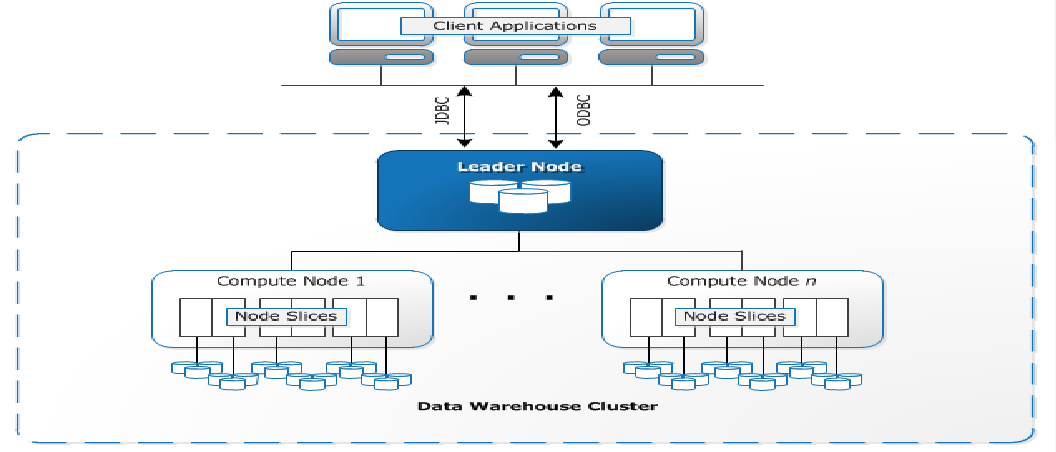
\includegraphics[width=\columnwidth]{images/amazon-architecture.png}
\caption{Architecture of Amazon Redshift data 
warehouse~\cite{hid-sp18-412-Amazon_Redshift_architecture}}\label{sa:archi}
\end{figure*}

	The amazon redshift data warehouse is a group of the nodes which
	act as a specific compute resource. These nodes are together grouped 
	and we call them as a cluster. The each of the cluster uses at 
	least one database, and in order to provide the processing unit 
	each of the cluster will have a Amazon redshift 
	engine~\cite{hid-sp18-412-Amazon_Redshift_architecture}.

	  A specific node in the cluster will be treated as the leader node and 
	  the rest of the other nodes as the compute nodes. The leader will 
	  be able to receive the requests from the client applications and
	  parse the queries and carries out the process of developing the 
	  query execution plan to fulfill the 
	  client request~\cite{hid-sp18-412-Amazon_Redshift_architecture}.
		
	\subsection{Client Applications}
	The most of the tools with respect to the data mining, analytics, 
	and the business intelligence reporting tools can be integrated into 
	Amazon Redshift, also including the ETL tools. The Amazon redshift is 
	constructed based on the industry-standard PostgreSQL, and this enables 
	the easy integration of the 
	business applications with the 
	Amazon Redshift~\cite{hid-sp18-412-Amazon_Redshift_architecture}.
        
	\subsection{Connections}
	 The most of the recent industry-standards PostgreSQL JDBC and the 
	 ODBC drivers are used for the communication between the client 
	 applications~\cite{hid-sp18-412-Amazon_Redshift_architecture}.
    
	\subsection{Clusters}
	 The major component of the Amazon Redshift is a cluster. 
	 A cluster contains other nodes which are called as the compute nodes. 
	 The coordination between these nodes is handled by the leader node. 
	 The leader node also interacts with the client application and all the 
	 internal communications are handled 
	 by the leader node~\cite{hid-sp18-412-Amazon_Redshift_architecture}. 
    
	\subsection{Leader Node}
	 The leader node acts as a leader in a team and effectively manages 
	 the communication between the client applications and compute nodes. 
	 The leader node compiles the code and will handle the distribution of 
	 the compiled code to the compute nodes. In order to run the complex 
	 queries, the leader node will parse and develop the execution plan 
	 with the specific number of steps and deliver the result to the 
	 request of the 
	 client application~\cite{hid-sp18-412-Amazon_Redshift_architecture}.
        
	The leader node will completely handle a query that needs to be 
	executed by the client application unless if there is reference 
	table residing on the compute node. In case, if there is a reference 
	table that resides on the compute node then the leader node will 
	distribute the SQL query to the compute node and complete the 
	execution by obtaining the result from the compute 
	node~\cite{hid-sp18-412-Amazon_Redshift_architecture}.
		
	\subsection{Compute Nodes}
	The compute nodes are in continuous coordination with the leader node. 
	The compute node performs the individual tasks that are assigned by the 
	leader node and executes the part of the query required by the leader 
	node. The compute nodes process the part of the compiled code that 
	is received from the leader node. They execute this part of the 
	compiled code and send these intermediate results 
	back to the 
	leader node~\cite{hid-sp18-412-Amazon_Redshift_architecture}.

    	Each of the compute nodes has an individual CPU, memory, and the disk 
	storage depending on the node type. The compute node can be upgraded 
	depending on the processing needs and the execution context that is 
	required for the execution of the client application. The cluster 
	capacity can also be increased by increasing the number of the 
	compute nodes that are allocated. Specifically, there are two types 
	of the nodes that are offered by the Amazon Redshift,  they are dense 
	storage nodes and the dense compute nodes. The storage capacity of a 
	single node can start from 160 GB and can extend up to the size of 
	16 TB~\cite{hid-sp18-412-Amazon_Redshift_architecture}.
        
	\subsection{Node Slices}
        The compute node is further partitioned into slices. 
		These slices are allocated a part of the computing memory 
		in order to process the part of the execution of the workload. 
		The distribution of the workload is managed by the leader node. 
		The slice concurrently executes to complete the execution of 
		the query assigned to 
		the main node~\cite{hid-sp18-412-Amazon_Redshift_architecture}.

\section{Key Features}
\label{s:keyf}
	This section discusses the key features of the Amazon redshift such 
	as Optimization of the Data warehousing, Petabyte Scale, No Up-Front 
	Costs, Fault Tolerant, Automated Backups etc.

	The diverse innovations enable the amazon redshift to perform 
	effectively with the queries ranging from the hundred gigabytes 
	to an exabyte or more. In order to process the local data with 
	the size of the petabyte, the amazon redshift uses the techniques 
	such as columnar storage, data compression and zone maps for the 
	effective reduction of the I/O to process the complex queries. 
	The architecture is designed to process the distributed SQL 
	operations with the goal of utilizing all the 
	resources~\cite{hid-sp18-412-Amazon_Redshift_Official_Page}.
		
	\subsection{Petabyte Scale}
	 The number of the nodes can be easily changed with the help of 
	 few button clicks in the AWS console. The number of the nodes 
	 can extend upto more than that contain petabytes of the user data 
	 can be handled effectively by the Amazon Redshift. 
	 The dense compute (DC) nodes will allow the users 
	 to create a high-performance data warehouses that have the fast CPUs, 
	 large amounts of RAM and high-speed Solid 
	 State Drive (SSD)~\cite{hid-sp18-412-Amazon_Redshift_Official_Page}. 
    
	\subsection{No Up-Front Costs}
	The pricing is based on the on-demand pricing with the less up-front 
	costs. This avoids the additional unnecessary costs incurred as 
	compared to the other platforms. The more details with respect to 
	the pricing are out of the scope of 
	this paper~\cite{hid-sp18-412-Amazon_Redshift_Official_Page}.
        
    \subsection{Serializable Isolation}
     In the distributed environment, some of the applications may not only 
	 require the concurrent querying and loading but also the functionality 
	 to write to the multiple tables parallel. To effectively provide this 
	 serializable isolation Amazon redshift has the support for the default 
	 automatic commit behavior which enables the SQL commands that are 
	 executed separately to be committed 
	 individually
	 ~\cite{hid-sp18-412-Amazon_Redshift_Serializable_Isolation}.
		
	\subsection{Automated Backups}
    	Amazon RDS has the ability to automatically backup the DB instance. 
	The storage volume snapshot of the DB instance can be easily created 
	to successively back up the complete  DB instance rather than each 
	database separately~\cite{hid-sp18-412-Amazon_Redshift_Official_Page}.
   
	 \subsection{Resize Progress Indicator}
	  This is the novel addition in the Amazon Redshift. The clusters 
	  size can be modified in Amazon Redshift, and the progress 
	  needs to be monitored. In order to effectively monitor the progress, 
	  Amazon redshift provides the redshift console as shown in the Figure 
	  ~\ref{sa:ind} in order to provide an efficient monitoring 
	  functionality for 
	  the users~\cite{hid-sp18-412-Features_Amazon_Redshift}.
	\label{sa:ind}
	\begin{figure}[!ht]
	\centering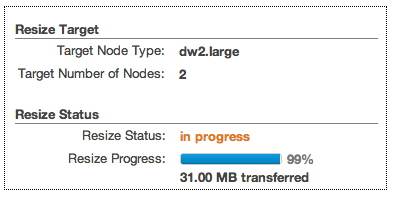
\includegraphics[width=\columnwidth]
	{images/resize-indicator.png}
	\caption{Resize Progress Indicator 
	Console~\cite{hid-sp18-412-Features_Amazon_Redshift}}\label{sa:ind}
	\end{figure}
	
\section{Comparison with Related Technologies}
\label{s:comp}
	\subsection{Compression Techniques}
	The techniques used for the compression of the data resembles the 
	technique that is used by the Vertica which is a column-oriented 
	database. The major difference between the Redshift is that it 
	skips the traditional indexes and rather the focus is made on the 
	sequential scan speed with the execution of the compiled code. 
	The column blocks are correctly skipped in order to increase the 
	scan speed depending on the values stored in 
	the memory~\cite{hid-sp18-412_Gupta_2015_ARC}.
        
	\subsection{Block Skipping Techniques}
	 The block skipping techniques used by the Amazon redshift is similar 
	 to the Infobright Knowledge grid and the Netezza’s Zone Maps which 
	 also rely on the same. The code compilation techniques used in the 
	 Amazon Redshift has been currently attracted to be used in the 
	 systems such as the Academia and 
	 Microsoft’s Hekaton~\cite{hid-sp18-412_Gupta_2015_ARC}.
        
	\subsection{Column Oriented DBMS Products}
	The amazon redshift’s core database technology was derived from the 
	technology licensed from ParAccel. The technologies such as the parser, 
	optimizer, engine, storage organization, MPP architecture that are 
	used in the Amazon Redshift were originally derived from the ParAccel 
	which is the Column-oriented DBMS product. At the end of 2000’s systems 
	such as Vertica, Ingres Vectorwise, Kickfire, Infobright and the 
	many of the other systems came into the picture that had the 
	same kind of the similarities with respect to the architecture and 
	the design. There included the same kind of the features that 
	were motivated by the two developing novel column-store 
	systems namely C-Store 
	and MonetDB/X100~\cite{hid-sp18-412_Gupta_2015_ARC}.

\section{License and Pricing}
\label{s:license}

	The Amazon redshift can be purchased and used with 
	the below three options:
	
	\begin{itemize}
	
	\item On-Demand Pricing 
	The cost will be based on the hourly rate with respect to 
	the type and the 
	number of nodes available 
	in the cluster~\cite{hid-sp18-412-Amazon_Redshift_Pricing}.
	
	\item Amazon Redshift Spectrum Pricing
	This pricing is mainly based on the number of bytes 
	scanned while running 
	the query~\cite{hid-sp18-412-Amazon_Redshift_Pricing}.
	
	\item Reserved Instance pricing
	This can be utilized to save up to 75% as compared to the 
	On-Demand rates while being dedicated to 
	be used for 
	1 or 3 year term~\cite{hid-sp18-412-Amazon_Redshift_Pricing}.
	
	\end{itemize}

\section{Conclusion}
\label{s:conclusion}
	Amazon Redshift is dedicated to helping all the 
	companies to upgrade and provide the cost-effective simple 
	service for the data warehousing. The advantages of the Amazon 
	redshift as compared to the traditional 
	data warehousing systems exceed to a great extent. With the easy and 
	simple mechanisms, it is possible to set-up a data-warehousing platform 
	avoiding the hassles of installation, tuning, and configuration.
    
    	Amazon redshift overcomes the price hurdles for the small and mid-sized 
	organizations that target to utilize the cloud-based data warehousing 
	solutions. Additionally, it also ensures the data durability and the 
	availability through the automatic replication and back-up via 
	Amazon S3 storage service. 
    
    	In the recent years, there has been an overwhelming number of the 
	enterprise's shifts from the native data-warehousing environment 
	to the cloud systems in order to leverage the benefits of the 
	cloud's accessibility and cost-effectiveness. With the goal 
	of providing the easy migration ability for these enterprise 
	models, AWS has enabled an effective warehousing solution as 
	compared to the traditional warehousing systems.  
	
\begin{acks}

  The author would like to thank Dr.~Gregor~von~Laszewski for his continous
  support and valuable suggestions to successfully complete this paper.
  
\end{acks}

\bibliographystyle{ACM-Reference-Format}
\bibliography{report} 
